\documentclass{article}
\author{Charlie}
\usepackage{graphicx} 
\usepackage{url}
\usepackage{amsmath}
\usepackage{amssymb}
\usepackage{geometry} 
\usepackage{asymptote}

\title{\vspace{-3cm}Stochastic Simulation}

\begin{document}

\newgeometry{margin=1in}


\section{Introduction}
While stochastic simulation has many applications and ideologies,
the goal in any simulation study is to evaluate estimators $\hat{\theta}$, 
of one or more parameters 
\begin{align}
    \theta = E\phi(X) \label{eq: expectation of loss function}
\end{align} 
where function $\phi(X)$ encodes the quantity or relationship we aim to evaluate 
on some domain $X$ \cite{alma9946168020001381}.
In a statistical application, $\phi(X)$ is some probabilistic model with input 
\textit{random variable} $X$,
where we wish to evaluate approximately how this model behaves.
Alternatively, $\phi(X)$ may be a completely deterministic function but is impossible or inefficient
to evaluate analytically, hence we aim to approximate its value through simulation.  
\\
In this chapter we delve into the latter case, and see how stochastic simulation 
is used in \textit{path tracing} to efficiently model the deterministic but complex nature 
of light particles in computer graphics.

\section{Path Tracing Model}

\begin{figure}[h]
    \centering
    \caption{Model of Path Tracing}
    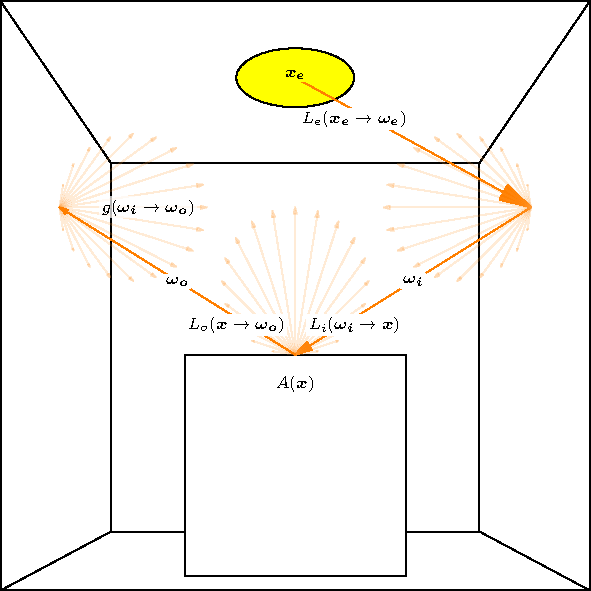
\includegraphics{path_tracing_model.pdf}
\end{figure}

As seen in Fig.() our \textit{path tracing} simulation is modeled as a 3D 
space with a single light emitter $e$.
That emitter projects rays with an \textit{incidence} direction vector $\boldsymbol{\omega_i}$
onto multiple planes $A$ at position vector $\boldsymbol{x}$.
The ray is then reflected with an \textit{outgoing} direction vector $\boldsymbol{\omega_o}$,
this path is defined as $(\boldsymbol{\omega_i}\rightarrow\boldsymbol{x}\rightarrow\boldsymbol{\omega_o})$.
The intensity of any given path is represented as $L_i(\boldsymbol{\omega_i}\rightarrow\boldsymbol{x})$
on incidence and $L_o(\boldsymbol{x}\rightarrow\boldsymbol{\omega_o})$ on outgoing, where 
$L_o=L_e$ at the emitter. 

At each reflection, the rays intensity is scaled down based on geometry and material variables.
For example, it is scaled by $1$ in a mirrors perfect reflection and $0$ in a true black's full absorption.
However, in this chapter to reduce complexity we will just assume this scaling to be calculated based on some
scattering term $g(\boldsymbol{\omega_i},\boldsymbol{\omega_o})$\label{fn: scattering term}.
\\
Hence, for a single light path from position $\boldsymbol{x}$ in direction $\boldsymbol{\omega_o}$,
we have
\begin{align}
    L_o^{single}(\boldsymbol{x}\rightarrow\boldsymbol{\omega_o}) 
    = L_e(\boldsymbol{x}\rightarrow\boldsymbol{\omega_o}) 
    + L_{i}^{single}(\boldsymbol{\omega_{i}}\rightarrow\boldsymbol{x})
    g(\boldsymbol{\omega_i},\boldsymbol{\omega_o})
\end{align}
where if $\boldsymbol{x}$ is a light source then $L_i=0$ as we are at the emitter and hence $L_o=L_e$.
Otherwise, if $\boldsymbol{x}$ is on a surface $A$ then $L_e=0$ assuming surface doesn't emit light.
Starting at the emitter $L_e$ this can be solved recursively all the way to solve for $L_o$ or vice versa.

However, this is only for a single path, any given $L_o$ will be the cumulation of many different 
incidence rays at position $\boldsymbol{x}$.
Thus, if we want the total contribution to $L_o$ from all possible incidence paths
we must integrate over all possible incidence light paths and their surface positions $A(\boldsymbol{x_i})$,
\begin{align} 
    \label{eq: equation of outgoing intensity}
    L_o(\boldsymbol{x}\rightarrow\boldsymbol{\omega_{o}}) = 
    L_e(\boldsymbol{x}\rightarrow\boldsymbol{\omega_o}) +
    \int_{A} L_{i}(\boldsymbol{\omega_{i}}\rightarrow\boldsymbol{x})
    g(\boldsymbol{\omega_i},\boldsymbol{\omega_o})
    \, dA(\boldsymbol{x_i}).
\end{align}
Once again, starting at the source we can solve each integral recursively to solve for $L_o$.
\\
 \begin{figure}[h]
    \centering
    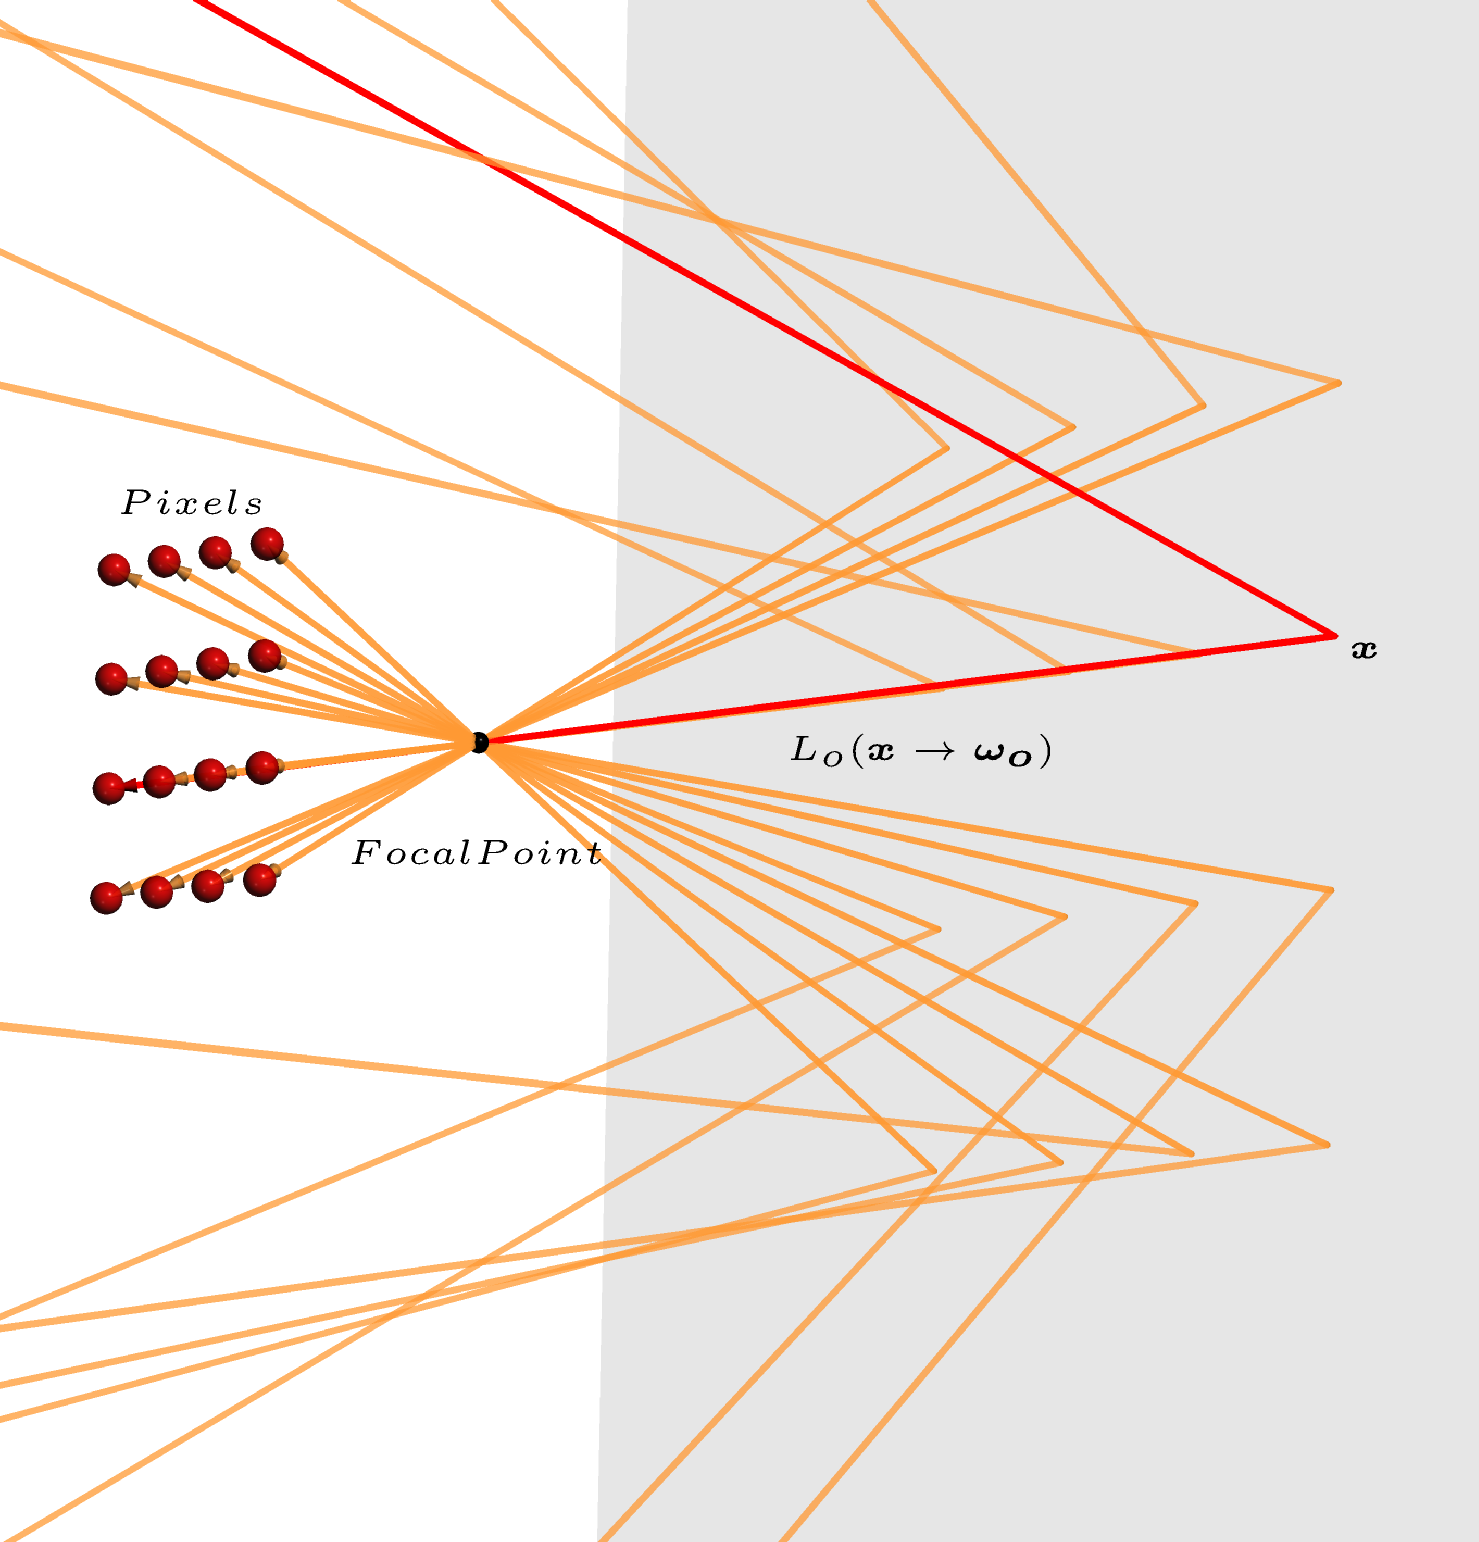
\includegraphics[width=0.5\linewidth]{model_of_lens.pdf}
    \caption{Shows the path of light into a pixel through a lens.}
    \label{fig:model of light through a lens}
\end{figure}
\\
Now imagine, we solve for the $L_o(\boldsymbol{x}\rightarrow\boldsymbol{\omega_o})$ that intersects 
with some virtual pixel after passing through a pinhole lense Fig().
It is clear, we now know what intensity to display that pixel at to produce realistic lighting of 
position $x$.
Repeating this process for all pixels, gives a perfect global illumination image of some virtual scene.  
This \textit{rendering equation} has no known closed-form solution and requires using \textit{Monte Carlo}
integration to evaluate. 
As shown in Eq.(\ref{eq: variance of importance sampling}) Monte Carlo integration has variance 
that reduces proportional to $1/N$ irrespective of the dimensions of an integral. 
For this reason it is the best way to approximate for $L_o$ in our path tracing simulation. \cite{KajiyaJamesT.1986Tre} 

\section{Monte Carlo Integration}
From Eq.(\ref{eq: equation of outgoing intensity}) it is not immediately evident 
how a stochastic simulation can be used to evaluate for the integral 
$L_o(\boldsymbol{x}\rightarrow\boldsymbol{\omega_o})$ on the domain $A$. 
\\
If we let some parameter $\theta$ be the integral of
$f(\boldsymbol{x})$
over domain $D \subset \mathbb{R}^d$,
where $\boldsymbol{x} = (x_1,\dots,x_d)$, then 
\begin{align}
    \theta &= \int_{D} f(\boldsymbol{x}) \, d\boldsymbol{x}. \notag \\
    \intertext{However, if we transform it to be an expected value for some random variable} \notag 
    &= \int_{D} \frac{f(\boldsymbol{x})}{p_X(\boldsymbol{x})}p_X(\boldsymbol{x}) \, d\boldsymbol{x}
    \intertext{where $p_X$ is the p.d.f. of $\boldsymbol{X}=(X_1,\dots,X_d)$ 
    and $p_X(\boldsymbol{x}) > 0$ when $f(\boldsymbol{x})\neq 0$, thus} \notag \\
    &=E \left[ \frac{f(\boldsymbol{X})}{p_X(\boldsymbol{X})} \right].
\end{align}
It can be seen that this is in the form of Eq.(\ref{eq: expectation of loss function}),
where $\theta$ is the parameter we are trying to solve for. 
Thus, in the same way we would for a stochastic model, we can solve this through random sampling by
taking the sample mean $\hat{\theta}$ as an unbiased estimator
\begin{align}
    \label{eq: general unbias sample mean}
    \hat{\theta} = \frac{1}{N} \sum_{i=1}^{N} \frac{f(\boldsymbol{X}_i)}{p_X(\boldsymbol{X}_i)}
\end{align}
where $\hat{\theta} \rightarrow \theta$ as $N \rightarrow \infty$.
\\
And thus it becomes clear that we can solve Eq.($\ref{eq: equation of outgoing intensity}$) by taking 
$N \rightarrow \infty$ random samples of the incidence rays with 
direction $\boldsymbol{\omega_i}$, from the random variable $\Omega$.
\begin{align}
    L_o(\boldsymbol{x}\rightarrow\boldsymbol{\omega_o}) &= \frac{1}{N} \sum_{i=1}^{N} \label{eq: sample mean of total paths}
    \frac{L_i(\boldsymbol{\omega_i}\rightarrow\boldsymbol{x})g(\boldsymbol{\omega_i},\boldsymbol{\omega_o})}
    {p_\Omega(\boldsymbol{\omega_i})}\\
    \intertext{Additionally, because it can be seen that $L_i$ can be solved by recursively
    applying Eq.(\ref{eq: sample mean of total paths}) until $L_i=L_e$ after $K_i$ steps, we have}
    &= \frac{1}{N} \sum_{i=1}^{N} \prod_{k=1}^{K_i} \left( \frac{1}{M} 
    \sum_{j=1}^{M} \frac{g(\boldsymbol{\omega_{k,j}},\boldsymbol{\omega_{k-1,j}})}
    {p_\Omega(\boldsymbol{\omega_{k,j}})} \right) L_e \label{eq: estimator for intensity with M samples}
\end{align}
where $k$ is our $k^{th}$ recursion and $j$ is our $j^{th}$ sample at the $k^{th}$ recursion.
Here we are assuming that we have the same sample size $M$ and p.d.f. $p_\Omega$ at each recursion, 
however even if they were different this would still be an un-bias estimator. 
In fact, often more complex algorithms adjust these variables proactively to reduce variance. 
\\
Here we let $M=1$, which despite increasing the variance, reduces computational requirements
and makes the model easier to visualise. 
\begin{align}
    L_o(\vec{x},\boldsymbol{\omega_o}) \label{eq: unbiased estimator for intesnity with M=1}
    &= \frac{1}{N} \sum_{i=1}^{N} \prod_{k=1}^{K_i} 
    \left( \frac{g(\boldsymbol{\omega_{k}},\boldsymbol{\omega_{k-1}})}
    {p_\Omega(\boldsymbol{\omega_{k}})} \right) L_e
\end{align}
Intuitively, this can be thought of as starting at some position $\boldsymbol{x}$
with an outgoing radiance $L_o$.
We then sample random variable $\Omega$ with p.d.f. $p_\Omega$ for a random
incidence direction $\boldsymbol{\omega_i}$.
We then backwards propagate through this path, repeating the process at every interaction with a surface,
until we reach the light source $L_e$. We then calculate the total scaling of $L_e$ by the scattering
terms $g(\boldsymbol{\omega_{k}},\boldsymbol{\omega_{k-1}})$, and being divided by $p_\Omega(\boldsymbol{\omega_k})$ to remove bias at every step. 
This scaled value of $L_e$ is one sample of $L_o$, where the sample mean is an estimator for $L_o$
that converges as $N\rightarrow\infty$.
This can be clearly seen as the recursive sampling in 
Eq.(\ref{eq: unbiased estimator for intesnity with M=1}).

\subsection{Importance Sampling}
While an estimator $\hat{\theta}$ is certainly unbias for any $p_X(x)$ as seen in 
Eq.(\ref{eq: general unbias sample mean}), it does not mean that the variance remains constant
regardless of what distribution we choose to sample with. 
In fact, it is apparent that our choice of $p_X$ weights our sample for values with a higher 
probability and thus with an optimal choice of p.d.f we can reduce the variance.
\\
Evaluating the variance of $\hat{\theta}$ from Eq.(\ref{eq: general unbias sample mean}), we have
\begin{align}
    var\,\hat{\theta} &= \frac{1}{N}\, var \left( \frac{f(\boldsymbol{X})}{p_X(\boldsymbol{X})} \right) \\
    &=\frac{1}{N} \left[ \,\,\, E \left( \frac{f^{2}(\boldsymbol{X})}{p_{X}^{2}(\boldsymbol{X})} 
    \right) - E\left( \frac{f(\boldsymbol{X})}{p_{X}(\boldsymbol{X})} \right)^{2} \,\,\, \right]\\
    &=\frac{1}{N} \left[ \,\,\, E \left( \frac{f^{2}(\boldsymbol{X})}{p_{X}^{2}(\boldsymbol{X})} 
    \right) - \theta^{2}\,\,\, \right].\label{eq: variance of importance sampling}
\end{align}
It can be clearly seen in Eq.(\ref{eq: variance of importance sampling}), that as $p_x(\boldsymbol{x})$
more closely resembles $|f(\boldsymbol{x})|$ the variance reduces. 
In fact, Jensen's inequality allows us to derive that our minimum variance occurs for 
$p_X(\boldsymbol{x}) \propto |f(\boldsymbol{x})|$ \cite{gentle2003random}.
\\
Fig() shows the clear advantage of a good sample distribution. 
\\
\\
Unsurprisingly, this is termed \textit{importance sampling} as we sample where we expect to get the most 
contribution to our final estimator.

Naturally, this can be applied to path tracing in a variety of ways. 
One obvious method is to sample with a distribution similar to the scattering term
$g(\boldsymbol{\omega_i}\rightarrow\boldsymbol{\omega_o})$ from section \ref{fn: scattering term}. 
Intuitively, this makes sense as sampling in areas with more light will provide a greater contribution 
to our final image as shown in Fig().

Another, basic method of importance sampling is deciding when to terminate a path. 
By terminating paths based on a p.d.f. that relates to the absorption probability of light,
we prevent wasted resources on long sample paths.
\\
Fig() shows path tracer algorithms with different levels of importance sampling for the same run time.

\section{Simulating Random Variables}

While it is clear that we can estimate complex integrals via estimating samples, 
the question of how to actually create these sample distributions still remains 
unanswered.

\subsection{Generating Random Numbers}

In simulation theory we define randomness as, events which are non-deterministic, independent 
and also follow a known distribution \cite{shiryaev2016probability}. 
Hence, the first step in simulating any random variable, is to generate a sequence of 
\textit{independent and identically distributed} random numbers.
\paragraph{True Random Numbers}
These are generated numbers that are in every essence truly non-deterministic and independent.
The only known method to generate such numbers is to measure inherently entropic natural phenomena.
This can include atomic decay, or the random state of internal hardware as measured by 
\textbf{HAVEGE} \cite{gentle2003random}.
However, no matter what the generator, in the case of simulation which requires computational algorithms,
outsourcing RNG is far to limiting to be viable. 

\subsubsection{Pseudorandom Numbers}
The caveat is that we only need random numbers to seem random within the framework of our model,
but the methods of generation can in fact be completely algorithmic. These deterministic generators 
are what are commonly referred to as \textit{pseudorandom number generators} or PNG \cite{alma9954732790001381}. 

\paragraph{Linear Congruential Generators}
By creating a \textit{true} random seed $x_0$ through \textbf{HAVEGE},
we can recursively use the algorithm denoted LCG[$m,a,c$] or equivalently
\begin{align} 
    \label{eq: Linear Congruential Generator}
    x_{i} \equiv (ax_{i-1} + c) \pmod{m},\quad\text{    with    }\quad0\leq x_{i}<m.
\end{align}
Thus, producing a \textit{Lehmer} sequence of uniformly distributed numbers with period $k \leq m$. 
We define parameters $a$, $c$ and $m$ as the \textit{multiplier}, \textit{increment} 
and \textit{modulus} respectively,
where in a \textit{multiplicative Congruential generator} the increment $c=0$. \cite{alma9954732790001381}\cite{gentle2003random}

A popular choice is \textit{the Minimal Standard} LCG[$2^{31}-1,16807,0$], which 
despite being deterministic can be seen in fig() to be an i.i.d.
$X \sim U(a,b)$ random variable \cite{HELLEKALEK1998485}.
\\
For every generator, there will exist applications in which the determinism of the generator
is exploited to introduce bias. However, often this can be mitigated by the correct choice of parameters.

\paragraph{Period}
It is generally accepted, that for linear methods an upper bound for the sample size is $n = \sqrt{k}$, 
where $k$ is the period of the PNG \cite{HELLEKALEK1998485}.
Thus methods to find and then maximise the period of a generator are necessary. 
For any LCG[$m,a,c=0$] the maximal period is bounded by the \textit{Euler totient function} $\phi(m)$,
occurring only when $a$ and $m$ are coprime. \cite{gentle2003random}.
Furthermore, it is evident from Eq.(\ref{eq: Linear Congruential Generator}) 
that the generator repeats for the smallest positive $k$ such that $x_{i} = x_{i+k}$.
Thus by solving recursively from $x_i$ till $x_{i+k}$ we have
\begin{align}
    a^{k} &\equiv 1\text{ mod }m,
\end{align}
where $k=\phi(m)$, if $a$ and $m$ are coprime. \cite{gentle2003random}

Thus in the minimal standard LCG, because $a=16807$ and $m=2^{31}$ are coprime,
our maximal period is $k=\phi(2^{31})=2^{31}-1$, which is large enough for most sample sizes.

\paragraph{Independence through Dimensions}
Additionally, we must ensure independence is maintained through the dimensions $d$ of our application.
In our path tracer Eq.(\ref{eq: unbiased estimator for intesnity with M=1}), 
every sample path of $k_i$ recursions has dimensions of at least $d=2K_i$. 
That means we need a PNG such that biases do not accumulate over every bounce in our simulation. 
We can clearly see in fig(), that despite \textit{the Minimal Standard} having
parameters that maximise the period, the distribution of $d$-tuples $x_n=(x_{n},x_{n+1}\dots x_{n+d})$
have a clear correlation in $d = 2$ \cite{HELLEKALEK1998485}. 
\\
This is a known weakness of LCGs as while they are efficient they have poor dimensionality.
For this reason path tracers such as ours commonly use the \textit{Mersenne Twister} generator, which has 
period $2^{19937}-1$, more than the number of photons that has ever existed,
and dimensions $d = 623$ potentially allowing for samples with upwards of $300$
bounces \cite{10.1145/272991.272995}. 

Fig() shows the comparison of the \textit{Minimal Standard} and the \textit{Mersenne Twister} 
in path tracing over 
equal sample size.

\subsection{Generating Random Variables}

\paragraph{The Inverse Transformation Method} Naturally once we have found a suitably un-bias 
linear generator we must simulate the desired distribution.

Let U be a uniform (0,1) random variable. 
Then for the monotone c.d.f. $F$ with inverse $F^{-1}$,
we define the random variable $X$ as
\begin{align}
	X&=F^{-1}(U).
\intertext{Thus}
    F_{X}(a)&=P\{X\leq a\} \\ \notag
    &=P\{F^{-1}(U)\leq a\} \\ \notag
    &=P\{U\leq F(a)\}\\ \notag
    &=F(a) \quad \cite{ross2007introduction}.  
\end{align}
\\
For a diffuse surface in path tracing, it is common to importance sample a cosine distribution to 
better simulate how Lambertian reflectance occurs. Fig() shows how a linear 
generator can generate a cosine transformation.

It should be noted that the theory for these equations assumes $U$ is a true random variable.
Hence, when using PNGs we must test our simulated random variable to be sure it is distributed 
correctly \cite{alma9946168020001381}.
In the case where independence has been confirmed, a given sample sequence that passes a significantly 
rigorous good-fit test against p.d.f. $p_X$ of $X$, can from then on be taken to be a sample from
random variable $X$ \cite{HELLEKALEK1998485}.  

\paragraph{Kolmogrov-Smirnov Test}

The Glivenko-Cantelli theorem states that,
for a random sample  $X_{1},\dots,X_{n}$ from some unknown c.d.f. $F_X(x)$,
and our \textit{sample c.d.f.} $F_N(x)$, defined as 
\begin{align}
F_{N}(x)=\frac{1}{N}(\text{number of $X_{i}$ less than or equal to $x$}) ~,
\end{align}
then
\begin{align}
\lim_{ N \to \infty } P\left[\sup_{x} |F_{N}(x)-F_{X}(x)|>\epsilon\right]  = 0 ~.
\end{align}
Thus showing for large N the maximum deviation
$\sup_{x} |F_{N}(x)-F_{X}(x)|$,
denoted simply as $D_N$, between the \textit{true} function $F_X$ and our sample c.d.f. $F_N$ is small 
for all $x$. 
Using this quality Kolmogrov proved and Smirnov later formalised that for any continuous
distribution $F_X$
\begin{align}
\lim_{ N \to \infty } P(\sqrt{ N }~D_{N}\leq x)=H(x)
\end{align}
where the Kolmogrov distribution function $H(x)$ is tabulated. 
Thus remarkably this Kolmogrov-Smirnov test allows a sample of any distribution and any 
sufficiently large sample size (at least 35) to be evaluated against $H(x)$. \cite{alma9954732790001381}

Fig() shows the comparison of the \textit{sample c.d.f.} $F_N(x)$ of our generated cosine random variable 
from Fig() against the Kolmogrov distribution function $H(x)$.




\bibliographystyle{plain}
\bibliography{references} 
\end{document}